\renewcommand{\theequation}{\theenumi}
\begin{enumerate}[label=\arabic*.,ref=\thesubsection.\theenumi]
\numberwithin{equation}{enumi}

%
\item Find the equation of the line $L$ joining the points 
\begin{align}
\vec{A}=\myvec{5 & -1 &4}^T
\\
\vec{B}=\myvec{4 & -1 & 3}^T
\end{align}
\solution The desired equation is
\begin{align}
\vec{x} &= \vec{B} + \lambda\brak{\vec{A}-\vec{B}}
\\
&= \myvec{4 \\ -1 \\ 3} + \lambda \myvec{1 \\ 0 \\ 1}
\label{eq:Lproj}
\end{align}
\item Plot the above line. 
\\
\solution The following code generates Fig. \ref{fig:3.1}.
\begin{lstlisting}
codes/3d/3.1.py
\end{lstlisting}
\begin{figure}[!ht]
\centering
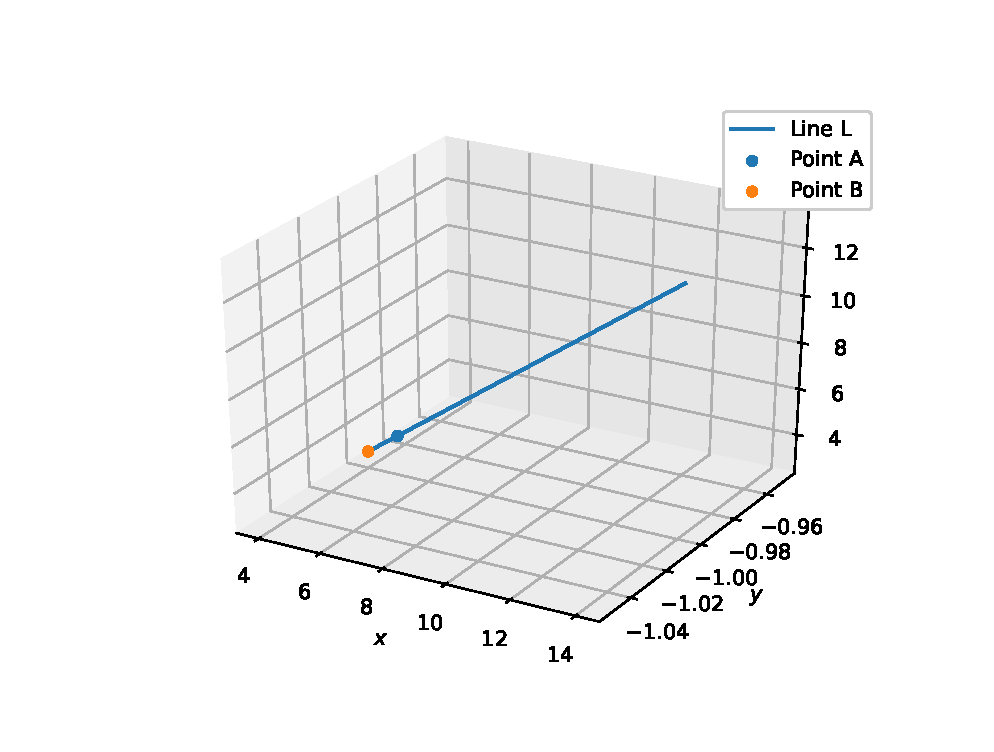
\includegraphics[width=\columnwidth]{./3d/figs/3.1.eps}
\caption{}
\label{fig:3.1}
\end{figure}
\item Find the intersection of $L$ and the plane $P$ given by
\begin{equation}
\myvec{1 & 1 & 1}\vec{x} = 7
\label{eq:Pproj}
\end{equation}
\\
\solution From \eqref{eq:Lproj} and \eqref{eq:Pproj},
\begin{align}
 \myvec{1 & 1 & 1}\myvec{4 \\ -1 \\ 3} + \lambda \myvec{1 & 1 & 1}
\myvec{1 \\ 0 \\ 1} &= 7
\\
\implies 6 + 2\lambda &= 7
\\
\implies \lambda &= \frac{1}{2}
\end{align}
%
Substituting in \eqref{eq:Lproj},
\begin{equation}
\vec{x} = \frac{1}{2}\myvec{9 & -1 & 7}
\end{equation}
\item Sketch the line, plane and the point of intersection.
\\
\solution The following code generates Fig. \ref{fig:3.2}.
\begin{lstlisting}
 
codes/3d/3.2.py
\end{lstlisting}
\begin{figure}[!ht]
\centering
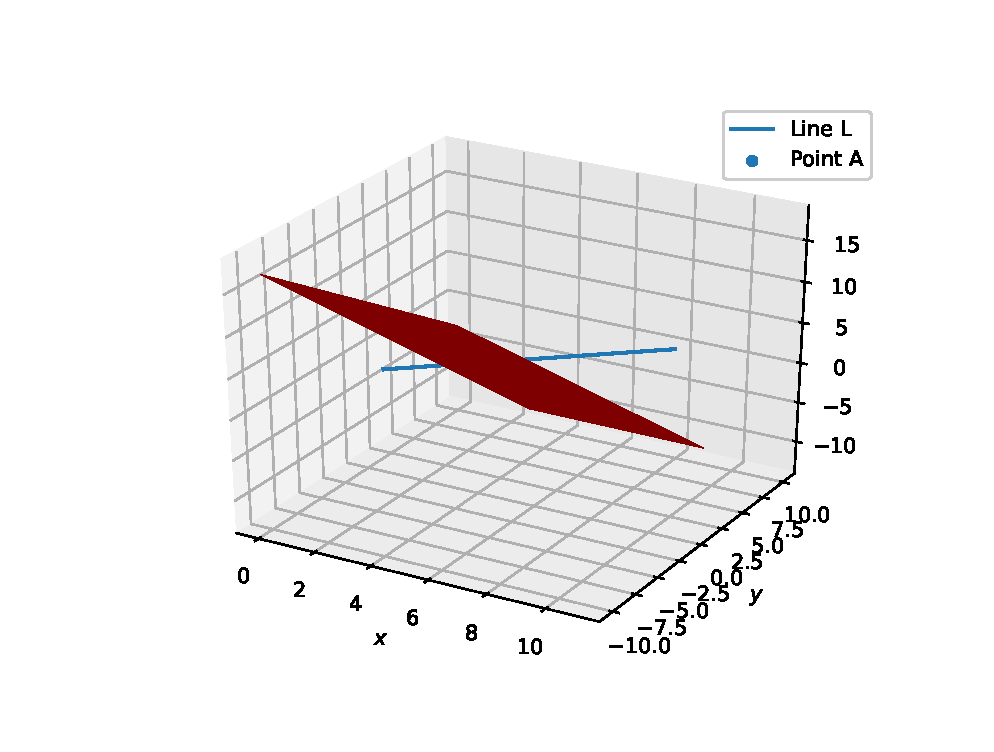
\includegraphics[width=\columnwidth]{./3d/figs/3.2.eps}
\caption{}
\label{fig:3.2}
\end{figure}
\item Find $\vec{C} \in P$  such that $AC \perp P$.  
\\
\solution From \eqref{eq:Pproj}, the direction vector of $AC$ is $\myvec{1 & 1 & 1}^T$.  Hence, the equation of 
$AC$ is
\begin{equation}
\vec{x} = \myvec{5 \\ -1 \\ 4} + \lambda_1  \myvec{1 \\ 1 \\ 1}
\end{equation}
Substituting in \eqref{eq:Pproj}
\begin{align}
 \myvec{1 & 1 & 1}\myvec{5 \\ -1 \\ 4} + \lambda \myvec{1 & 1 & 1}
\myvec{1 \\ 1 \\ 1} &= 7
\\
\implies 8 + 3\lambda_1 &= 7
\\
\implies \lambda_1 &= -\frac{1}{3}
\end{align}
Thus,
\begin{align}
\vec{C} = \frac{1}{3}\myvec{14 \\ -4 \\ 11}
\end{align}
%\item Summarize the above through a plot.
%\\
%\solution The following code generates Fig. \ref{fig:3.3}.
%\begin{lstlisting}
% 
%codes/3d/3.3.py
%\end{lstlisting}
%\begin{figure}[!ht]
%\centering
%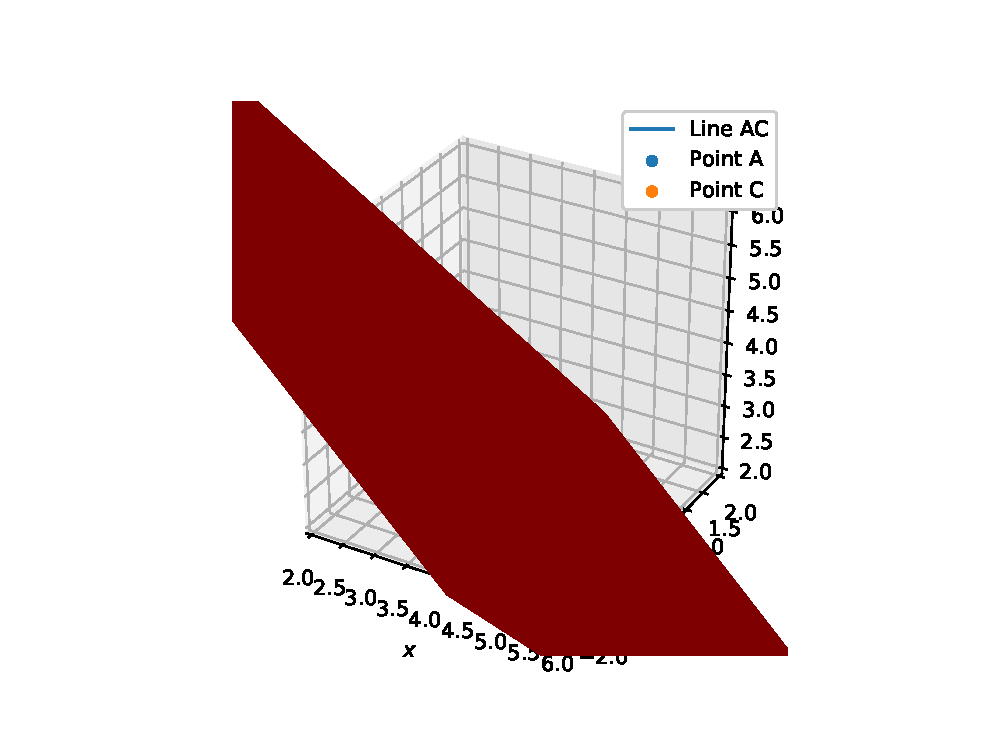
\includegraphics[width=\columnwidth]{./3d/figs/3.3.eps}
%\caption{}
%\label{fig:3.3}
%\end{figure}
\item Show that if $BD \perp P$  such that $\vec{D} \in P$,
\begin{equation}
\vec{D} = \frac{1}{3}\myvec{13 \\ -2 \\ 10}
\end{equation}
%
\item Find the projection of $AB$ on the plane $P$.
\\
\solution The projection is given by
\begin{align}
CD = \norm{\vec{C}-\vec{D}} = \sqrt{\frac{2}{3}}
%\label{eq:homog}
\end{align}
\item Show that the projection of $\vec{x}$ on $\vec{y}$ is
\begin{align}
\label{eq:2019_qp2_14_proj}
\frac{\vec{x}^T\vec{y}}{\norm{\vec{y}}^2}\vec{y}
\end{align}
\end{enumerate}
